\chapter{Epidemiología del cáncer}

La epidemiología se ha definido tradicionalmente como la ciencia que estudia la distribución y los determinantes de la enfermedad en los seres humanos \cite{MacMahon1970}. En una definición más moderna, no limitada exclusivamente a la enfermedad, la epidemiología se define como el estudio de la aparición y distribución de los estados o acontecimientos relacionados con la salud en poblaciones específicas, incluyendo el estudio de los determinantes de estos estados y la aplicación del conocimiento al control de los problemas de la salud \cite{Porta2008}.

\section{Indicadores epidemiológicos}

Para medir en la población el impacto del cáncer se utilizan principalmente cuatro indicadores:

\begin{itemize}
	\item \textbf{Incidencia} (casos nuevos). Mide el riesgo de presentar cáncer.
	\item \textbf{Mortalidad} (defunciones). Mide el riesgo de morir por cáncer.
	\item \textbf{Supervivencia} (porcentaje de casos vivos). Mide la historia natural del cáncer y efectividad del tratamiento.
	\item \textbf{Prevalencia} (casos nuevos y antiguos, vivos). Mide la carga asistencial de la enfermedad.
\end{itemize}

Además, se puede examinar la evolución de cada indicador a lo largo del tiempo, hablando así de tendencias de la incidencia, de la mortalidad, de la supervivencia o de la prevalencia.\\

% ---------------------------------

\section{Fuentes de información}

A nivel mundial, las estadísticas de incidencia, mortalidad y prevalencia de cáncer las proporciona el \textit{Global Cancer Observatory} (GCO), una plataforma web de la \textit{International Agency for Research on Cancer}, de la Organización Mundial de la Salud \cite{Bray2018, GCO}. El organismo equivalente al GCO a nivel europeo es el \textit{European Cancer Information System} (ECIS), de reciente creación y apoyado por la Comisión Europea \cite{ECIS, ECIS2}. Para conocer la supervivencia, el programa CONCORD \cite{Allemani2018} publica datos a nivel mundial y EUROCARE \cite{DeAngelis2014} a nivel europeo.\\

Aunque estos organismos proporcionan estadísticas sobre cáncer en España, también existen fuentes a nivel nacional que cuentan con datos más actualizados y con distinta metodología. La Red Española de Registros de Cáncer (REDECAN) publica periódicamente datos sobre incidencia y supervivencia de cáncer en España \cite{REDECAN2020, Guevara2019}, mientras que las estadísticas de mortalidad por cáncer se pueden calcular a partir de las defunciones que publica el Ministerio de Sanidad, Consumo y Bienestar Social (MSCBS) del Gobierno de España \cite{MSCBS} y la población que proporciona el Instituto Nacional de Estadística \cite{INEpob}.

% ---------------------------------

\section{Incidencia de cáncer}

\subsection{Metodología}

Para medir de manera precisa la incidencia de cáncer en una población es necesaria la existencia de un Registro de Cáncer Poblacional. Estas entidades se dedican a registrar exhaustivamente todos los casos de cáncer diagnosticados en un área geográfica y sus datos son muy útiles para todo tipo de estudios epidemiológicos. Algunos de estos Registros cubren la población de todo un país (por ejemplo, Canadá) mientras que otros cubren regiones concretas (por ejemplo, la provincia de Granada). Desgraciadamente, muchas áreas geográficas no están cubiertas por un Registro de Cáncer Poblacional. Es el caso de España, en el que sólo el 27\% de la población está cubierta por un Registro de Cáncer Poblacional \cite{Redondo-Sanchez2019}. Para conocer de manera estimada la incidencia de cáncer en territorios sin Registro de Cáncer Poblacional o proyectar la incidencia a años posteriores se utilizan diversos métodos matemáticos y estadísticos \cite{Bray2018, GCO, ECIS, ECIS2, REDECAN2020, Redondo-Sanchez2019}.\\

Con respecto a las medidas usadas para reportar la incidencia, la más sencilla y fácil de interpretar es el número nuevo de casos de cáncer, enmarcado siempre en un periodo concreto de tiempo y un área geográfica. A partir del número de casos se puede calcular la tasa bruta (TB), un indicador que tiene en cuenta el tamaño de la población y que se suele calcular por 100.000 habitantes \cite{IARC1995}.\\

$$\text{TB}  = 100.000 \cdot \dfrac{\text{Número de casos nuevos}}{\text{Personas en riesgo}}$$\\

Para permitir comparaciones entre distintas poblaciones, o la misma población en momentos distintos, es necesario tener en cuenta la estructura de edad de la población. Para responder a esta motivación se define la tasa estandarizada por edad (TE) como aquella tasa que habría en la población de estudio si tuviese exactamente la misma estructura de edad que una población estándar predefinida \cite{IARC1995}. La definición de la tasa estandarizada por edad para 18 grupos de edad quinquenales (0-4 años, 5-9 años, $\dots$, 80-84 años, 85 años y más) es la siguiente:

$$\text{TE} = \sum_{i = 1}^{18} \omega_i \dfrac{N_i}{P_i} $$
donde $N_i$ y $P_i$ son respectivamente el número de casos incidentes y la población en el $i$-ésimo grupo de edad, y $\omega_i$ es el peso que toma la población de referencia en el grupo $i$-ésimo, con $\sum_{i = 1}^{18}\omega_i = 100.000$. Los valores de ${\omega_i}$ están predefinidos en base a poblaciones estándar, siendo las más utilizadas en nuestro contexto las siguientes:

\begin{itemize}
	
	\item Población mundial. Propuesta por primera vez en 1960 \cite{SegiM.1960} y modificada más tarde en 1966 \cite{Doll1966}, permite realizar comparaciones a nivel mundial.
		
	\item Antigua población estándar europea. Propuesta en 1976 \cite{Waterhouse1976} basándose en la estructura de edad de varias poblaciones escandinavas, permite comparaciones entre zonas europeas.
	
	\item Nueva población estándar europea. En el año 2013, la Oficina Europea de Estadística (EUROSTAT) realiza una revisión de la población estándar europea con el objetivo de que la población refleje fielmente el envejecimiento existente en la población europea \cite{EUROSTAT2013}. Debido a su novedad, el uso de esta población aún no está ampliamente extendido en los organismos internacionales \cite{ECIS2} y en ocasiones se reportan las dos tasas estandarizadas por las poblaciones estándar antigua y nueva \cite{ECIS}.

\end{itemize}

En la Tabla 1 se muestran los pesos para cada una de las poblaciones de referencia mencionadas anteriormente.\\

%\newpage
\textbf{Tabla 1}. Pesos de las poblaciones estándar para el cálculo de tasas estandarizadas por edad.
\begin{table}[!htb]
	\begin{tabular}{|r|r|r|r|}
		\hline		
		Grupo de edad  &  \begin{tabular}[r]{@{}r@{}}Población estándar\\ mundial\end{tabular}  &  \begin{tabular}[r]{@{}r@{}}Población estándar\\ europea 1976\end{tabular}  &  \begin{tabular}[r]{@{}r@{}}Población estándar\\ europea 2013\end{tabular}\\\hline
		
		0-4 años  &  12.000  &  8.000  &  5.000\\
		5-9 años  &  10.000  &  7.000  &  5.500\\
		10-14 años  &  9.000  &  7.000  &  5.500\\
		15-19 años  &  9.000  &  7.000  &  5.500\\
		20-24 años  &  8.000  &  7.000  &  6.000\\
		25-29 años  &  8.000  &  7.000  &  6.000\\
		30-34 años  &  6.000  &  7.000  &  6.500\\
		35-39 años  &  6.000  &  7.000  &  7.000\\
		40-44 años  &  6.000  &  7.000  &  7.000\\
		45-49 años  &  6.000  &  7.000  &  7.000\\
		50-54 años  &  5.000  &  7.000  &  7.000\\
		55-59 años  &  4.000  &  6.000  &  6.500\\
		60-64 años  &  4.000  &  5.000  &  6.000\\
		65-69 años  &  3.000  &  4.000  &  5.500\\
		70-74 años  &  2.000  &  3.000  &  5.000\\
		75-79 años  &  1.000  &  2.000  &  4.000\\
		80-84 años  &  500  &  1.000  &  2.500\\
		$\geq$85 años  &  500  &  1.000  &  2.500\\\hline
	\end{tabular}
\end{table}

Para utilizar notación internacional, la tasa estandarizada por la población mundial se notará TE-M (población mundial), la tasa estandarizada por la población europea de 1976 se notará TE-aE (antigua población europea) y la de 2013 se notará TE-nE (nueva población europea).

\subsection{Incidencia del total del cáncer excepto piel no melanoma}

El cáncer de piel no melanoma se suele excluir al reportar datos de incidencia del total del cáncer debido a que es muy frecuente y cuenta con buen pronóstico, por lo que no se suele registrar en los Registros de Cáncer Poblacionales \cite{Gordon2013, Madan2010}.\\

Para dar una perspectiva global del cáncer y sus diferentes tipos, en la Figura 3 se muestran las localizaciones anatómicas más frecuentes de cáncer en el mundo, así como su distribución por sexos.

\begin{center}
	\textbf{Figura 3}. Gráfico de mosaico con la incidencia estimada de cáncer excepto piel no melanoma en el mundo para el año 2018. Ocho localizaciones anatómicas más frecuentes en ambos sexos. Fuente: \textit{Global Cancer Observatory}, Organización Mundial de la Salud \cite{GCO}.
\end{center}
\begin{center}
	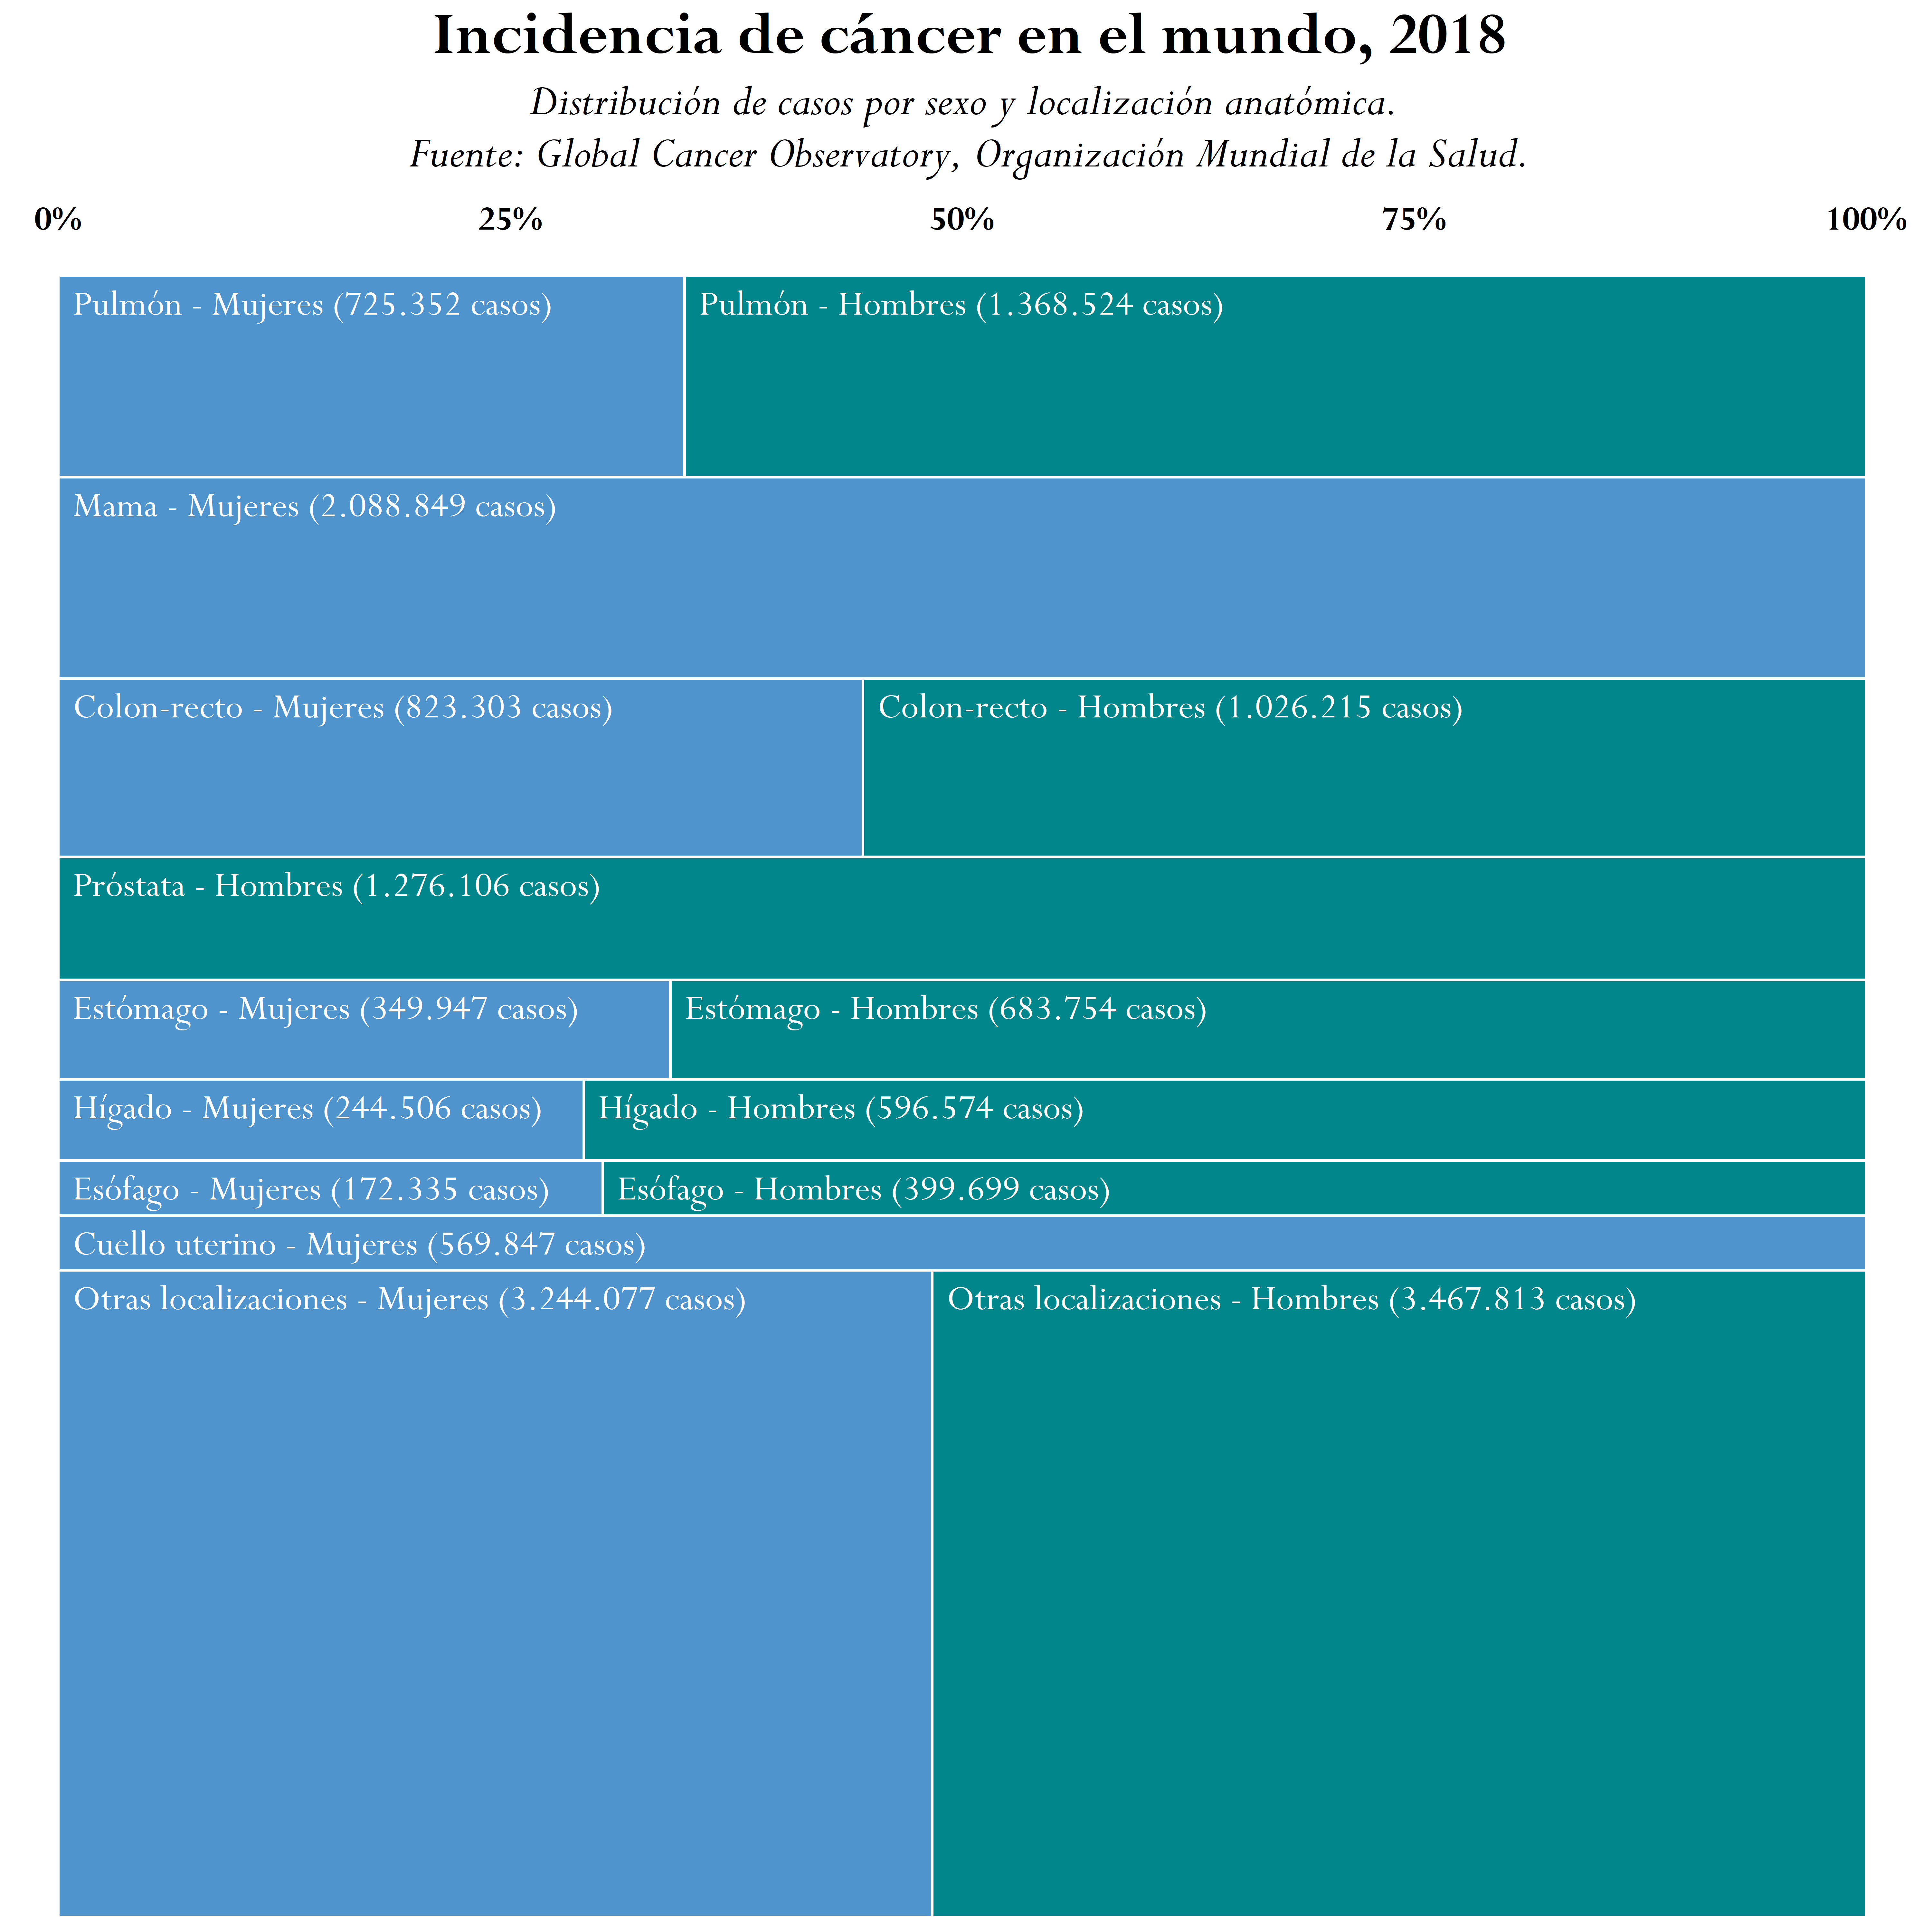
\includegraphics[width=.85\textwidth]{figuras/03_marimekko_gco_incidencia.png} 
\end{center}

El cáncer de pulmón es el más frecuente en todo el mundo, seguido por los cánceres de mama, colon-recto, próstata, estómago, hígado, esófago y cuello uterino. En la mayoría de las localizaciones anatómicas, el cáncer es más frecuente en hombres que en mujeres (Figura 3).\\

\newpage
\textbf{Tabla 2}. Incidencia del total del cáncer excepto piel no melanoma en 2018, por sexo y población. Número de casos nuevos (N), tasa bruta (TB), tasa estandarizada por la población mundial (TE-M),  tasa estandarizada por la antigua población europea (TE-aE) y  tasa estandarizada por la nueva población europea (TE-nE).

\begin{table}[H]
	\begin{tabular}{|c|l|c|r|r|r|r|r|}
		\hline		

		\multicolumn{1}{|c|}{Sexo} & \multicolumn{1}{|c|}{Población} & Fuente & \multicolumn{1}{|c|}{N} & \multicolumn{1}{|c|}{TB} & \multicolumn{1}{|c|}{TE-M} & \multicolumn{1}{|c|}{TE-aE} & \multicolumn{1}{|c|}{TE-nE}\\\hline
		
		\multirow{3}{*}{Hombres} & Mundo & GCO \cite{GCO} & 8.818.685 & 229,0 & 204,7 &  & \\
		& Europa & ECIS \cite{ECIS} & 2.059.673 & 572,9 & 302,7 & 436,0 & 651,7\\
		& España & ECIS \cite{ECIS} & 142.353 & 625,6 & 309,7 & 444,7 & 658,6\\\hline
		\multirow{3}{*}{Mujeres} & Mundo & GCO \cite{GCO} & 8.218.216 & 217,3 & 175,6 &  & \\
		& Europa & ECIS \cite{ECIS} & 1.851.644 & 481,8 & 242,7 & 332,6 & 451,2\\
		& España & ECIS \cite{ECIS} & 106.647 & 451,1 & 218,4 & 298,5 & 401,7\\\hline
		\multirow{3}{*}{\begin{tabular}[c]{@{}c@{}}Ambos\\sexos\end{tabular}} & Mundo & GCO \cite{GCO} & 17.036.901 & 223,2 & 187,8 &  & \\
		& Europa & ECIS \cite{ECIS} & 3.911.317 & 525,8 & 266,7 & 374,3 & 531,9\\
		& España & ECIS \cite{ECIS} & 249.000 & 536,7 & 259,4 & 363,8 & 515,3\\\hline
	\end{tabular}
\end{table}

A nivel nacional, REDECAN ha publicado estimaciones de la incidencia en España más recientes a las mostradas en la Tabla 2, correspondientes al año 2020 \cite{REDECAN2020}. En este análisis se estima el número de casos de cáncer excepto piel no melanoma en 277.394 casos (57,8\% en hombres), con una tasa bruta de 588,0 por 100.000 habitantes y tasas estandarizadas de 280,3 (TE-M), 399,4 (TE-aE) y 579,8 (TE-nE).

\subsection{Incidencia de cáncer de hígado}

El cáncer de hígado es el sexto cáncer más frecuente del mundo (Figura 3), con más de 840.000 casos nuevos anuales en todo el mundo, 82.000 de ellos en Europa y 6.600 en España (Tabla 3). Es un cáncer más frecuente en hombres que en mujeres: por cada caso en mujeres hay 2,4 casos en hombres. En ambos sexos, la TE-M de España (6,5) es mayor que la de Europa (5,1) aunque mucho menor que la del mundo (9,3).\\

\newpage
\textbf{Tabla 3}. Incidencia de cáncer de hígado en 2018, por sexo y población. Número de casos nuevos (N), tasa bruta (TB), tasa estandarizada por la población mundial (TE-M),  tasa estandarizada por la antigua población europea (TE-aE) y  tasa estandarizada por la nueva población europea (TE-nE).

\begin{table}[H]
	\begin{tabular}{|c|l|c|r|r|r|r|r|}
		\hline		
		
		\multicolumn{1}{|c|}{Sexo} & \multicolumn{1}{|c|}{Población} & Fuente & \multicolumn{1}{|c|}{N} & \multicolumn{1}{|c|}{TB} & \multicolumn{1}{|c|}{TE-M} & \multicolumn{1}{|c|}{TE-aE} & \multicolumn{1}{|c|}{TE-nE}\\\hline
		
		\multirow{3}{*}{Hombres} & Mundo & GCO \cite{GCO} & 596.574 & 15,5 & 13,9 &  & \\
		& Europa & ECIS \cite{ECIS} & 55.825 & 15,5 & 8,0 & 11,7 & 17,7\\
		& España & ECIS \cite{ECIS} & 4.976 & 21,9 & 10,9 & 15,7 & 22,5\\\hline
		\multirow{3}{*}{Mujeres} & Mundo & GCO \cite{GCO} & 244.506 & 6,5 & 4,9 &  & \\
		& Europa & ECIS \cite{ECIS} & 26.641 & 6,9 & 2,7 & 4,0 & 6,3\\
		& España & ECIS \cite{ECIS} & 1.654 & 7,0 & 2,4 & 3,6 & 6,0\\\hline
		\multirow{3}{*}{\begin{tabular}[c]{@{}c@{}}Ambos\\sexos\end{tabular}} & Mundo & GCO \cite{GCO} & 841.080 & 11,0 & 9,3 &  & \\
		& Europa & ECIS \cite{ECIS} & 82.466 & 11,1 & 5,1 & 7,4 & 11,3\\
		& España & ECIS \cite{ECIS} & 6.630 & 14,3 & 6,5 & 9,3 & 13,6\\\hline
				
	\end{tabular}
\end{table}

En las estimaciones publicadas por REDECAN para 2020 se estiman en España 6.595 casos de cáncer de hígado (75,4\% en hombres), con una tasa bruta de 14,0 y tasas estandarizadas de 6,5 (TE-M), 9,4 (TE-aE) y 13,9 (TE-nE) \cite{REDECAN2020}.

\subsection{Incidencia de cáncer de colon-recto}

El cáncer de colon-recto es el tercer cáncer más frecuente del mundo (Figura 3), con más de 1.800.000 casos nuevos anuales en todo el mundo. En Europa y España es el cáncer más frecuente en ambos sexos con 510.000 casos anuales en Europa y 37.000 en España (Tabla 4). Es un cáncer ligeramente más frecuente en hombres que en mujeres: por cada caso en mujeres hay 1,2 casos en hombres. En ambos sexos, la TE-M de España (81,1) es mayor que la de Europa (68,8) y la del mundo (24,2), lo que puede deberse a una mayor exposición a factores de riesgo como el tipo de dieta o la ausencia de un programa de cribado a nivel nacional \cite{Zavoral2009}.\\

\newpage
\textbf{Tabla 4}. Incidencia de cáncer de colon-recto en 2018, por sexo y población. Número de casos nuevos (N), tasa bruta (TB), tasa estandarizada por la población mundial (TE-M),  tasa estandarizada por la antigua población europea (TE-aE) y  tasa estandarizada por la nueva población europea (TE-nE).

\begin{table}[H]
	\begin{tabular}{|c|l|c|r|r|r|r|r|}
		\hline		
		
		\multicolumn{1}{|c|}{Sexo} & \multicolumn{1}{|c|}{Población} & Fuente & \multicolumn{1}{|c|}{N} & \multicolumn{1}{|c|}{TB} & \multicolumn{1}{|c|}{TE-M} & \multicolumn{1}{|c|}{TE-aE} & \multicolumn{1}{|c|}{TE-nE}\\\hline
		
		\multirow{3}{*}{Hombres} & Mundo & GCO \cite{GCO} & 1.026.215 & 26,6 & 23,6 &  & \\
		& Europa & ECIS \cite{ECIS} & 275.519 & 76,6 & 38,1 & 56,8 & 88,9\\
		& España & ECIS \cite{ECIS} & 23.013 & 101,1 & 45,8 & 68,5 & 107,2\\\hline
		\multirow{3}{*}{Mujeres} & Mundo & GCO \cite{GCO} & 823.303 & 21,8 & 16,3 &  & \\
		& Europa & ECIS \cite{ECIS} & 236.101 & 61,4 & 25,2 & 37,0 & 56,3\\
		& España & ECIS \cite{ECIS} & 14.642 & 61,9 & 23,6 & 34,9 & 53,5\\\hline
		\multirow{3}{*}{\begin{tabular}[c]{@{}c@{}}Ambos\\sexos\end{tabular}} & Mundo & GCO \cite{GCO} & 1.849.518 & 24,2 & 19,7 &  & \\
		& Europa & ECIS \cite{ECIS} & 511.620 & 68,8 & 30,8 & 45,6 & 70,0\\
		& España & ECIS \cite{ECIS} & 37.655 & 81,1 & 33,9 & 50,4 & 77,5\\\hline
	\end{tabular}
\end{table}

En las estimaciones publicadas por REDECAN para 2020 se estiman en España 44.231 casos de cáncer de colon-recto (58,9\% en hombres), con una tasa bruta de 93,8 y tasas estandarizadas de 40,0 (TE-M), 59,5 (TE-aE) y 91,9 (TE-nE) \cite{REDECAN2020}.

\section{Mortalidad por cáncer}

\subsection{Metodología}

Los indicadores para medir la mortalidad por cáncer son los mismos que para la incidencia, cambiando número de casos por defunciones por cáncer. Es importante destacar que la mortalidad por cáncer es por definición aquella mortalidad que es causada directamente por el cáncer. En este sentido, una persona diagnosticada de cáncer que falleciese por otras causas no puede ser considerada como fallecida por cáncer, sino fallecida con cáncer.\\

Aunque ECIS \cite{ECIS} reporta mortalidad por cáncer en España para el año 2018, la mortalidad que se presenta a continuación a nivel nacional es la que proporciona el MSCBS del Gobierno de España \cite{MSCBS}, ya que se consideran datos más fiables al tratarse de datos observados basados en certificados médicos de defunción y no ser estimaciones.
 
\subsection{Mortalidad del total del cáncer excepto piel no melanoma}

En el mundo se producen más de 9 millones de defunciones por cáncer anualmente, siendo esta enfermedad la segunda causa de muerte a nivel global, por detrás de las enfermedades cardiovasculares. Una de cada 6 muertes es causa directa del cáncer \cite{WorldHealthOrganization2018}.\\

Considerando ambos sexos conjuntamente, los cánceres que provocan más defunciones son los de pulmón, colon-recto y estómago, mientras que en mujeres el cáncer con más defunciones es el cáncer de mama y en hombres el de pulmón (Figura 4).

\begin{center}
\textbf{Figura 4}. Gráfico de mosaico con la mortalidad estimada por cáncer excepto piel no melanoma en el mundo para el año 2018. Ocho localizaciones anatómicas con más defunciones en ambos sexos. Fuente: \textit{Global Cancer Observatory}, Organización Mundial de la Salud \cite{GCO}.
\end{center}
\begin{center}
	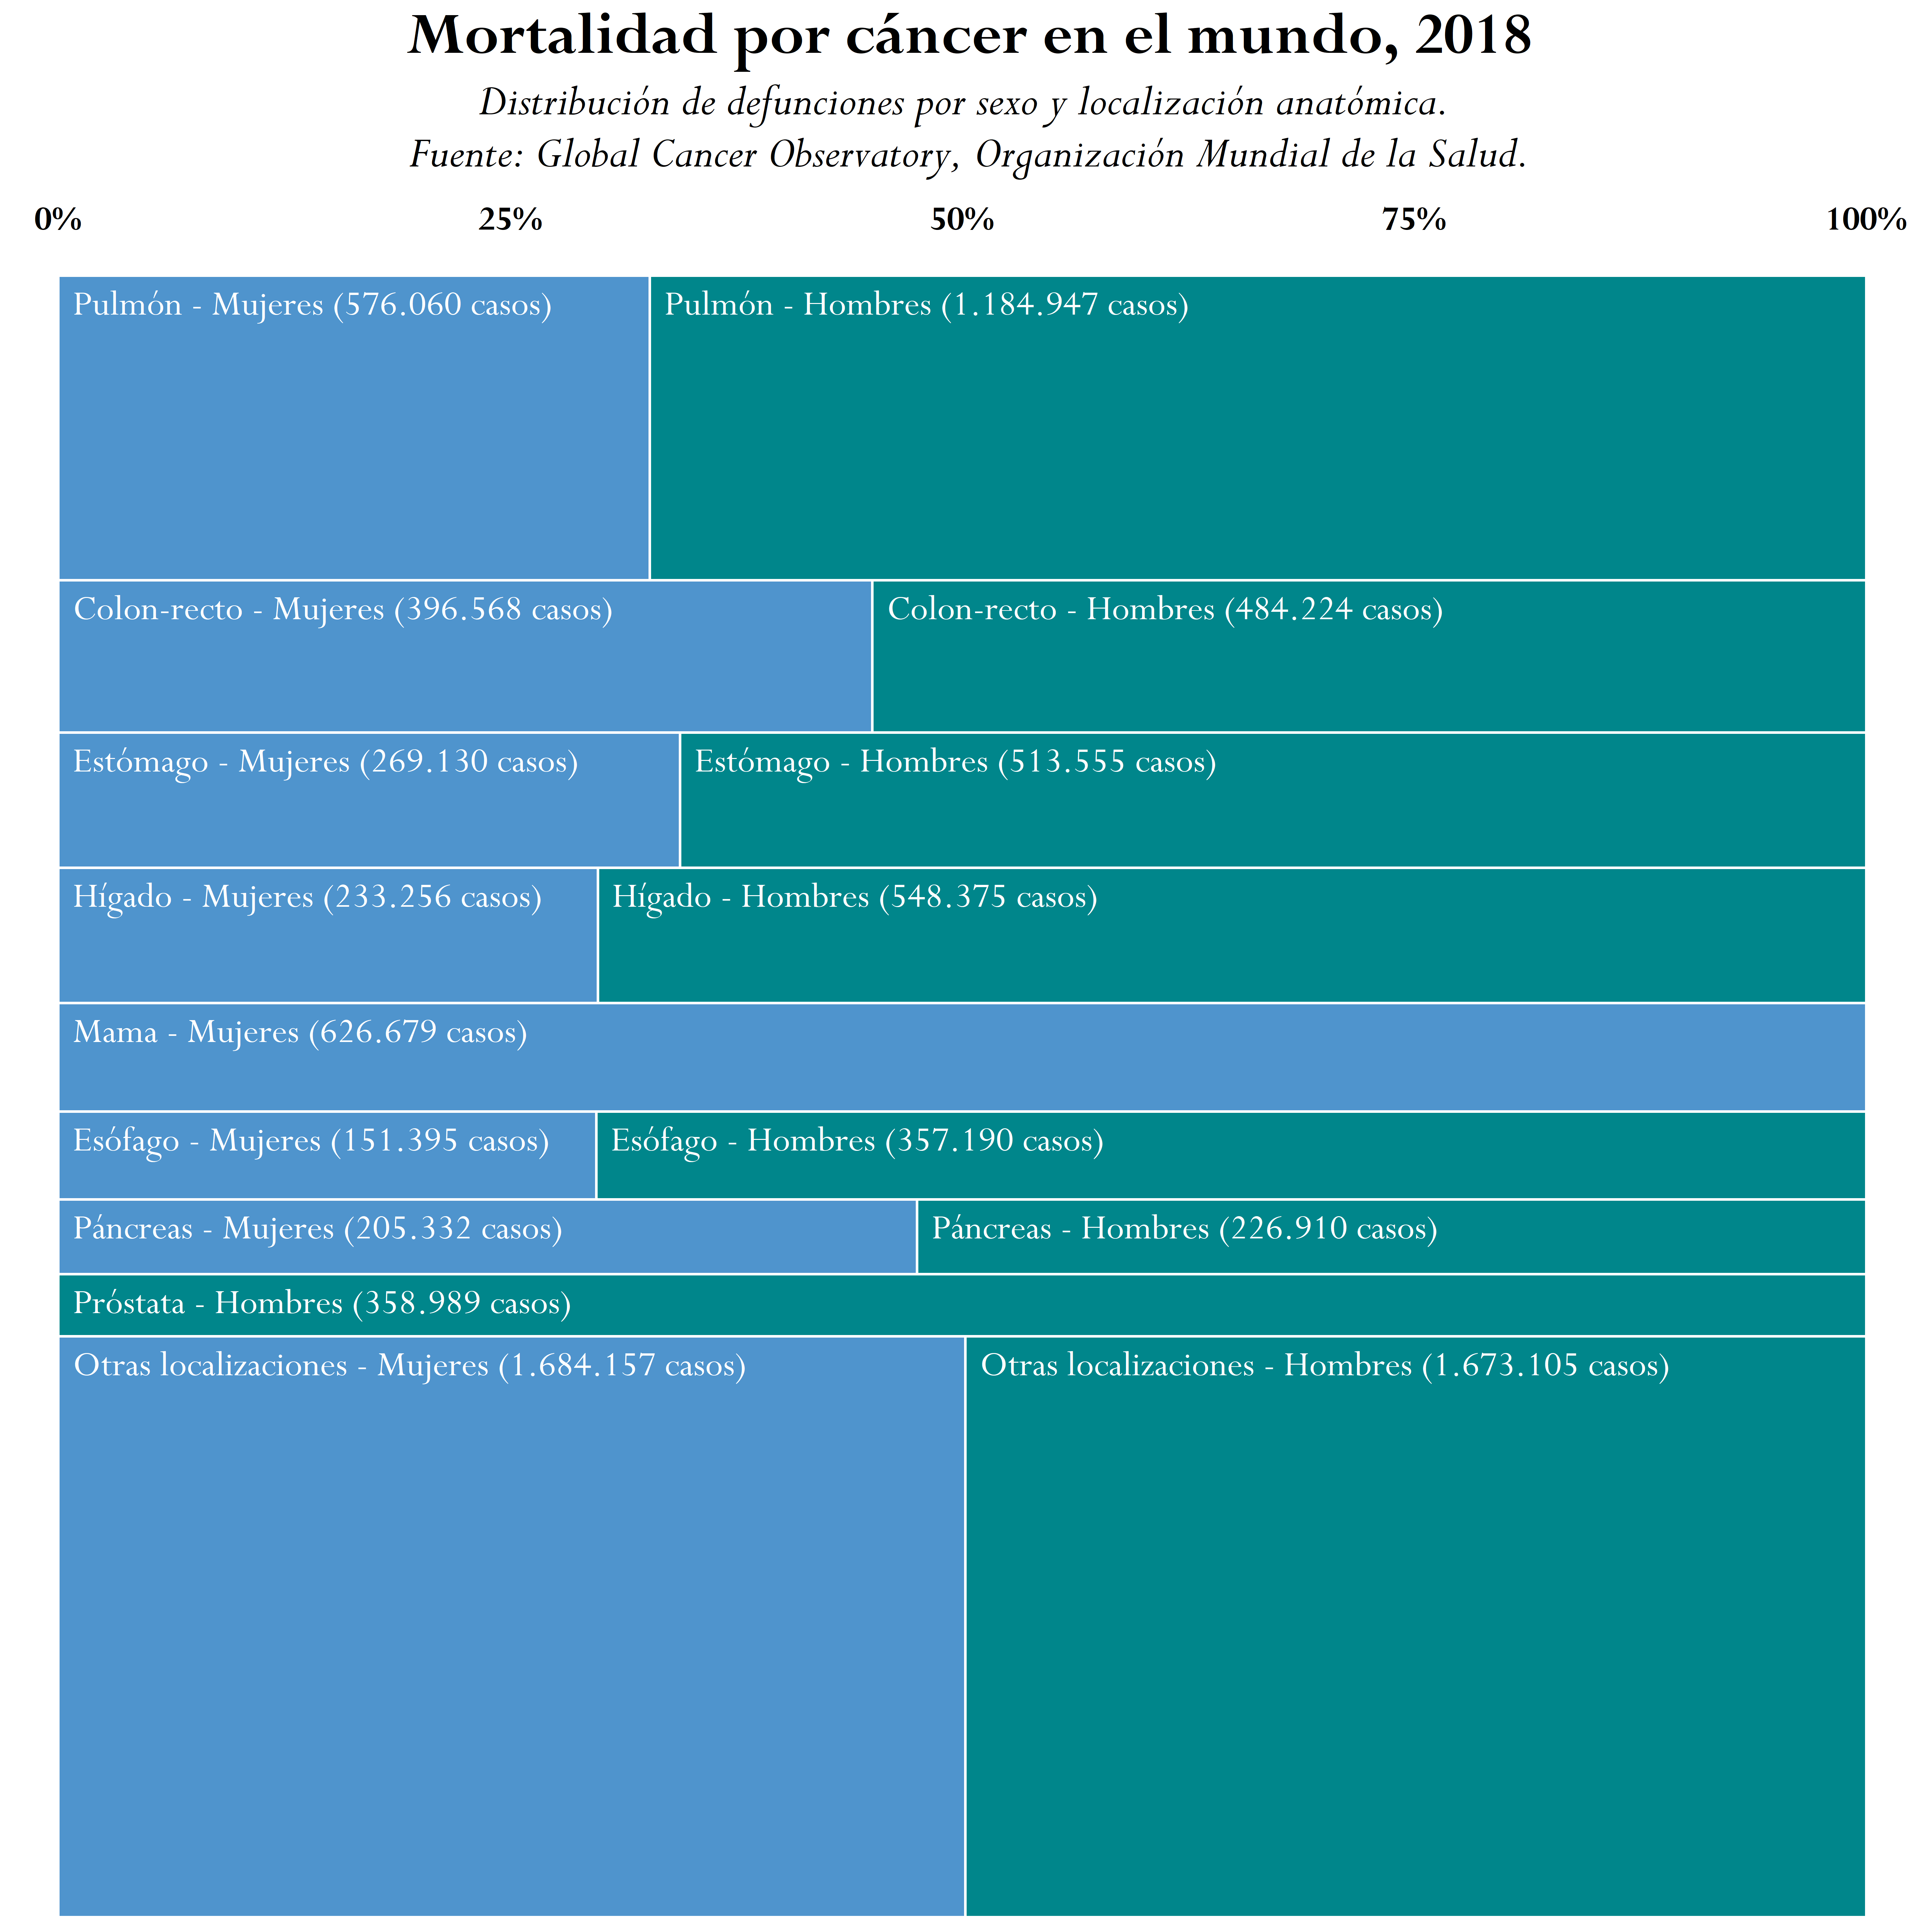
\includegraphics[width=.85\textwidth]{figuras/04_marimekko_gco_mortalidad.png} 
\end{center}

En España se producen más de 100.000 muertes anuales por cáncer, siendo la tasa de mortalidad inferior a la europea y a la mundial tanto en ambos sexos como en hombres y mujeres (Tabla 5).\\

\textbf{Tabla 5}. Mortalidad por total del cáncer excepto piel no melanoma en 2018, por sexo y población. Número de defunciones (N), tasa bruta (TB), tasa estandarizada por la población mundial (TE-M),  tasa estandarizada por la antigua población europea (TE-aE) y  tasa estandarizada por la nueva población europea (TE-nE).

\begin{table}[H]
	\begin{tabular}{|c|l|r|r|r|r|r|r|}
		\hline		
		
		\multicolumn{1}{|c|}{Sexo} & \multicolumn{1}{|c|}{Población} & \multicolumn{1}{|c|}{Fuente} & \multicolumn{1}{|c|}{N} & \multicolumn{1}{|c|}{TB} & \multicolumn{1}{|c|}{TE-M} & \multicolumn{1}{|c|}{TE-aE} & \multicolumn{1}{|c|}{TE-nE}\\\hline
		
		\multirow{3}{*}{Hombres} & Mundo & GCO \cite{GCO} & 5.347.295 & 138,9 & 121,9 &  & \\
		& Europa & ECIS \cite{ECIS} & 1.077.986 & 299,8 & 143,2 & 217,4 & 355,4\\
		& España & MSCBS \cite{MSCBS} & 65.610 & 286,4 & 121,3 & 186,8 & 314,1\\\hline
		\multirow{3}{*}{Mujeres} & Mundo & GCO \cite{GCO} & 4.142.577 & 109,5 & 82,7 &  & \\
		& Europa & ECIS \cite{ECIS} & 851.723 & 221,6 & 86,4 & 128,1 & 201,0\\
		& España & MSCBS \cite{MSCBS} & 42.248 & 177,4 & 63,2 & 94,6 & 151,1\\\hline
		\multirow{3}{*}{\begin{tabular}[c]{@{}c@{}}Ambos\\sexos\end{tabular}} & Mundo & GCO \cite{GCO} & 9.489.872 & 124,3 & 100,5 &  & \\
		& Europa & ECIS \cite{ECIS} & 1.929.709 & 259,4 & 110,8 & 165,8 & 263,9\\
		& España & MSCBS \cite{MSCBS} & 107.858 & 230,8 & 89,4 & 135,4 & 221,2\\\hline

	\end{tabular}
\end{table}


\subsection{Mortalidad de cáncer de hígado}

Si bien el cáncer de hígado es el sexto cáncer más incidente del mundo, en mortalidad ocupa la cuarta posición, siendo la causa de 782.000 defunciones anuales (Figura 4). La muerte por cáncer de hígado es mucho más frecuente en hombres que en mujeres. En Europa el cáncer de hígado causa cerca de 80.000 muertes y en España unas 5.100, con unas tasas de mortalidad muy similares y por debajo de la tasa mundial (Tabla 6).\\

\textbf{Tabla 6}. Mortalidad por cáncer de hígado en 2018, por sexo y población. Número de defunciones (N), tasa bruta (TB), tasa estandarizada por la población mundial (TE-M),  tasa estandarizada por la antigua población europea (TE-aE) y  tasa estandarizada por la nueva población europea (TE-nE).


\begin{table}[H]
	\begin{tabular}{|c|l|r|r|r|r|r|r|}
		\hline		
		\multicolumn{1}{|c|}{Sexo} & \multicolumn{1}{|c|}{Población} & \multicolumn{1}{|c|}{Fuente} & \multicolumn{1}{|c|}{N} & \multicolumn{1}{|c|}{TB} & \multicolumn{1}{|c|}{TE-M} & \multicolumn{1}{|c|}{TE-aE} & \multicolumn{1}{|c|}{TE-nE}\\\hline
		
		\multirow{3}{*}{Hombres} & Mundo & GCO \cite{GCO} & 548.375 & 14,2 & 12,7 &  & \\
		& Europa & ECIS \cite{ECIS} & 50.365 & 14,0 & 6,8 & 10,3 & 16,4\\
		& España & MSCBS \cite{MSCBS} & 3.577 & 15,6 & 7,0 & 10,7 & 17,0\\\hline
		\multirow{3}{*}{Mujeres} & Mundo & GCO \cite{GCO} & 233.256 & 6,2 & 4,6 &  & \\
		& Europa & ECIS \cite{ECIS} & 27.010 & 7,0 & 2,4 & 3,8 & 6,3\\
		& España & MSCBS \cite{MSCBS} & 1.564 & 6,6 & 2,0 & 3,2 & 5,6\\\hline
		\multirow{3}{*}{\begin{tabular}[c]{@{}c@{}}Ambos\\sexos\end{tabular}} & Mundo & GCO \cite{GCO} & 781.631 & 10,2 & 8,5 &  & \\
		& Europa & ECIS \cite{ECIS} & 77.375 & 10,4 & 4,4 & 6,6 & 10,6\\
		& España & MSCBS \cite{MSCBS} & 5.141 & 11,0 & 4,4 & 6,7 & 10,7\\\hline

		
	\end{tabular}
\end{table}

\subsection{Mortalidad de cáncer de colon-recto}

El cáncer de colon-recto es el segundo cáncer que provoca más defunciones, con más de 880.000 defunciones anuales en todo el mundo (Figura 4). La defunción por cáncer de colon-recto es ligeramente más frecuente en hombres que en mujeres. Las tasas de mortalidad en España y Europa son muy similares, por encima en ambos casos de la tasa mundial (Tabla 7).\\

\textbf{Tabla 7}. Mortalidad por cáncer de colon-recto en 2018, por sexo y población. Número de defunciones (N), tasa bruta (TB), tasa estandarizada por la población mundial (TE-M),  tasa estandarizada por la antigua población europea (TE-aE) y  tasa estandarizada por la nueva población europea (TE-nE).


\begin{table}[H]
	\begin{tabular}{|c|l|r|r|r|r|r|r|}
		\hline		
		
		\multicolumn{1}{|c|}{Sexo} & \multicolumn{1}{|c|}{Población} & \multicolumn{1}{|c|}{Fuente} & \multicolumn{1}{|c|}{N} & \multicolumn{1}{|c|}{TB} & \multicolumn{1}{|c|}{TE-M} & \multicolumn{1}{|c|}{TE-aE} & \multicolumn{1}{|c|}{TE-nE}\\\hline
		
		\multirow{3}{*}{Hombres} & Mundo & GCO \cite{GCO} & 484.224 & 12,6 & 10,8 &  & \\
		& Europa & ECIS \cite{ECIS} & 131.155 & 36,5 & 16,4 & 25,7 & 44,3\\
		& España & MSCBS \cite{MSCBS} & 9.222 & 40,3 & 15,8 & 25,1 & 44,4\\\hline
		\multirow{3}{*}{Mujeres} & Mundo & GCO \cite{GCO} & 396.568 & 10,5 & 7,2 &  & \\
		& Europa & ECIS \cite{ECIS} & 115.059 & 29,9 & 10,0 & 15,6 & 26,6\\
		& España & MSCBS \cite{MSCBS} & 6.066 & 25,5 & 7,5 & 11,9 & 20,7\\\hline
		\multirow{3}{*}{\begin{tabular}[c]{@{}c@{}}Ambos\\sexos\end{tabular}} & Mundo & GCO \cite{GCO} & 880.792 & 11,5 & 8,9 &  & \\
		& Europa & ECIS \cite{ECIS} & 246.214 & 33,1 & 12,8 & 19,9 & 33,8\\
		& España & MSCBS \cite{MSCBS} & 15.288 & 32,7 & 11,2 & 17,7 & 30,9\\\hline
	
	\end{tabular}
\end{table}

% ---------------------------------


\section{Supervivencia de cáncer} 

El proyecto CONCORD (\textit{Global surveillance of cancer survival}), coordinado por la \textit{London School of Hygiene \& Tropical Medicine}, es el mayor proyecto de investigación sobre supervivencia a nivel mundial. En su tercera y última publicación, se analizaron datos de más de 37 millones de pacientes procedentes de 322 Registros de Cáncer Poblacionales de 71 países \cite{Allemani2018}. Las tendencias de la supervivencia están aumentando con el tiempo, aunque se aprecian importantes diferencias entre territorios. Para casos de España diagnosticados durante el periodo 2010-2014, la supervivencia relativa estandarizada por edad a 5 años del diagnóstico es del 63,2\% para cáncer de colon, 59,5\% para cáncer de recto y 17,3\% para cáncer de hígado \cite{Allemani2018}.\\

En el contexto europeo, EUROCARE (\textit{European Cancer Registry based study on survival and care of cancer patients}) proporciona datos para el periodo 2000-2007, estimando la supervivencia relativa estandarizada por edad a 5 años del total del cáncer en un 50,3\% para hombres y 58,0\% para mujeres \cite{DeAngelis2014,ECIS}. Para cáncer de colon-recto la supervivencia es similar a la media global (54,7\% en hombres, 56,7\% en mujeres), y para cáncer de hígado la supervivencia es muy baja (11,5\% tanto para hombres como para mujeres) \cite{DeAngelis2014,ECIS}.\\

Los datos más recientes de supervivencia para España corresponden al periodo 2008-2013 y están publicados por REDECAN \cite{Guevara2019}. Para el total del cáncer excepto piel no melanoma, la supervivencia relativa estandarizada por edad a 5 años es de 55,3\% en hombres y 61,7\% en mujeres. El cáncer de hígado tiene una de las supervivencias más bajas, tanto en hombres (17,9\%) como en mujeres (16,2\%). La supervivencia del cáncer de colon es de 63,1\% en hombres y 63,9\% en mujeres, ligeramente superior que la supervivencia del cáncer de recto (60,4\% y 62,7\% para hombres y mujeres respectivamente).  

% ---------------------------------


\section{Prevalencia de cáncer}

En el mundo hay más de 11 millones de casos prevalentes de cáncer a 1 año, esto es, casos de cáncer en pacientes vivos que fueron diagnosticados en el último año \cite{GCO}. A 5 años el número se eleva hasta casi 39 millones de casos \cite{GCO}. En la Tabla 8 se muestra la prevalencia a 1 y 5 años por sexos y población para los cánceres de hígado y colon-recto, así como para el total del cáncer excepto piel no melanoma.\\

\newpage

\textbf{Tabla 8}. Prevalencia del total del cáncer excepto piel no melanoma, cáncer de hígado y cáncer de colon-recto en 2018, por sexo y población. Número de casos prevalentes y tasas por 100.000 habitantes a 1 y 5 años.

\begin{table}[H]
	\begin{tabular}{|c|c|c|rr|rr|}
		%\cline{4-7}
		\hline
		
			 &  &  & \multicolumn{2}{c}{1 año} & \multicolumn{2}{|c|}{5 años} \\\hline
			 &  &  & \multicolumn{1}{c}{N} & \multicolumn{1}{c|}{Tasa} & \multicolumn{1}{c}{N} & \multicolumn{1}{c|}{Tasa} \\ \hline

\multirow{9}{*}{\begin{tabular}[c]{@{}c@{}}Total del cáncer\\excepto piel no\\melanoma\end{tabular}} & \multirow{3}{*}{Hombres} & Mundo & 5.607.801 & 145,6 & 17.895.356 & 464,7\\
&  & Europa & 1.504.232 & 418,4 & 5.086.515 & 1414,7\\
&  & España & 105.599 & 464,0 & 356.427 & 1566,3\\ \cline{2-7}
& \multirow{3}{*}{Mujeres} & Mundo & 5.688.175 & 150,4 & 20.738.064 & 548,3\\
&  & Europa & 1.434.849 & 373,4 & 5.417.680 & 1409,8\\
&  & España & 84.409 & 357,0 & 322.341 & 1363,5\\ \cline{2-7}
& \multirow{3}{*}{\begin{tabular}[c]{@{}c@{}}Ambos\\sexos\end{tabular}} & Mundo & 11.295.976 & 148,0 & 38.633.420 & 506,1\\
&  & Europa & 2.939.081 & 395,1 & 10.504.195 & 1412,2\\
&  & España & 190.008 & 409,5 & 678.768 & 1462,9\\ \hline
\multirow{9}{*}{Hígado} & \multirow{3}{*}{Hombres} & Mundo & 236.669 & 6,1 & 471.525 & 12,2\\
&  & Europa & 21.240 & 5,9 & 39.867 & 11,1\\
&  & España & 1.924 & 8,5 & 3.618 & 15,9\\ \cline{2-7}
& \multirow{3}{*}{Mujeres} & Mundo & 97.621 & 2,6 & 203.685 & 5,4\\
&  & Europa & 9.719 & 2,5 & 18.610 & 4,8\\
&  & España & 580 & 2,5 & 1.102 & 4,7\\ \cline{2-7}
& \multirow{3}{*}{\begin{tabular}[c]{@{}c@{}}Ambos\\sexos\end{tabular}} & Mundo & 334.290 & 4,4 & 675.210 & 8,8\\
&  & Europa & 30.959 & 4,2 & 58.477 & 7,9\\
&  & España & 2.504 & 5,4 & 4.720 & 10,2\\ \hline
\multirow{9}{*}{Colon-recto} & \multirow{3}{*}{Hombres} & Mundo & 749.774 & 19,5 & 2.595.326 & 67,4\\
&  & Europa & 213.233 & 59,3 & 748.455 & 208,2\\
&  & España & 18.059 & 79,4 & 63.593 & 279,5\\ \cline{2-7}
& \multirow{3}{*}{Mujeres} & Mundo & 606.377 & 16,0 & 2.194.309 & 58,0\\
&  & Europa & 178.969 & 46,6 & 655.422 & 170,6\\
&  & España & 11.463 & 48,5 & 42.121 & 178,2\\ \cline{2-7}
& \multirow{3}{*}{\begin{tabular}[c]{@{}c@{}}Ambos\\sexos\end{tabular}} & Mundo & 1.356.151 & 17,8 & 4.789.635 & 62,8\\
&  & Europa & 392.202 & 52,7 & 1.403.877 & 188,7\\
&  & España & 29.522 & 63,6 & 105.714 & 227,8\\ \hline
	\end{tabular}
\end{table}







